\section{Архитектура решения}

\subsection{Общая структура системы}

Разрабатываемая в работе система построена как последовательный исследовательский конвейер, в котором каждый этап решает
отдельную подзадачу и передаёт результат следующему этапу через устойчивые артефакты. Такой подход позволяет отделить
подготовку данных от обучения моделей, оценку качества --- от интерпретации, а предиктивное ядро --- от
демонстрационного пользовательского слоя. В результате архитектура решения имеет модульный характер: система не сводится
к одной модели, а состоит из нескольких взаимосвязанных уровней, каждый из которых выполняет собственную функцию.

\begin{figure}[htbp]
    \centering
    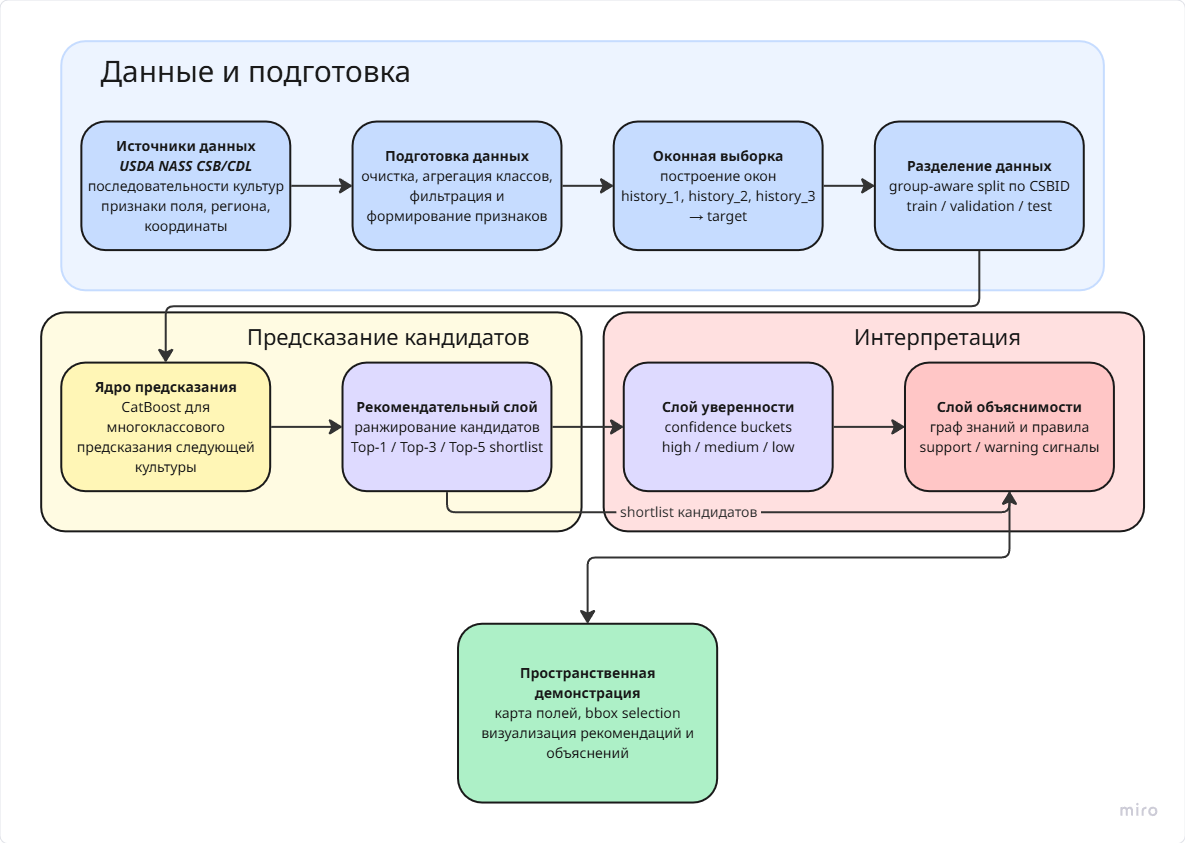
\includegraphics[width=0.95\textwidth]{figures/architecture.png}
    \caption{Общая архитектура предложенной рекомендательной системы}
    \label{fig:system_architecture}
\end{figure}

На рисунке~\ref{fig:system_architecture} показана общая последовательность этапов: от исходных данных USDA NASS CSB/CDL
и подготовки оконной выборки до формирования рекомендаций, оценки уверенности, интерпретации результатов и
пространственной демонстрации.

Архитектура построена вокруг последовательной передачи артефактов между этапами. После подготовки данных формируется
оконная выборка, используемая для обучения модели. Результатом работы предиктивного ядра является распределение
вероятностей по классам культур. На его основе формируется ранжированный список кандидатов, который затем дополняется
оценкой уверенности и интерпретационными признаками. Завершающий слой использует эти артефакты для визуального
представления результата.

Содержательно архитектура решения включает следующие уровни:

\begin{itemize}
\tightlist
\item
  уровень данных;
\item
  уровень подготовки и представления выборки;
\item
  уровень предиктивной модели;
\item
  уровень рекомендаций;
\item
  уровень уверенности;
\item
  уровень интерпретации рекомендаций;
\item
  уровень пространственной демонстрации.
\end{itemize}

Каждый из этих уровней будет кратко рассмотрен далее.

\subsection{Уровень данных и подготовки выборки}

Нижний уровень архитектуры образуют исходные данные USDA NASS CSB/CDL и процедуры их подготовки. На этом уровне решаются
задачи чтения исходного массива, сопоставления кодов культур, фильтрации нерелевантных классов и формирования рабочего
представления данных. Именно здесь закладывается основа всей последующей системы, поскольку от способа подготовки данных
зависит и качество модели, и интерпретируемость результата.

После базовой очистки данные преобразуются из годовых последовательностей в оконную выборку. Каждое наблюдение
представляется как переход от истории культур за несколько предыдущих лет к целевой культуре следующего года. В
рассматриваемой работе это представление имеет вид

\begin{equation}
\notag
(c_{t-3}, c_{t-2}, c_{t-1}) \rightarrow c_t
\end{equation}

где \(c_{t-3}\), \(c_{t-2}\) и \(c_{t-1}\) обозначают культуры на поле в три предыдущих года, а \(c_t\) --- целевую
культуру следующего года.

Такое преобразование позволяет перейти от исходной таблицы по годам к задаче предсказания следующего шага в
последовательности культур.
На этом же уровне выполняется фильтрация редких целевых классов и фиксируется итоговое пространство культур, с которым
далее работают все последующие компоненты системы.

Таким образом, уровень подготовки данных выполняет две основные функции. Во-первых, он делает данные пригодными для
машинного обучения. Во-вторых, он задаёт единый и воспроизводимый входной контракт для всех последующих этапов. Это
особенно важно, поскольку в работе сравниваются разные подходы, и такое сравнение возможно только при использовании
общей, заранее зафиксированной выборки.

\subsection{Предиктивное ядро}

Центральным элементом архитектуры является предиктивное ядро, задача которого --- по истории культур и дополнительным
признакам поля оценить вероятности следующих культур. В качестве основной предиктивной модели в работе используется
CatBoost. Выбор именно этой модели связан с тем, что задача имеет табличную природу и включает как категориальные, так
и числовые признаки. В рамках архитектуры CatBoost рассматривается как предиктивное ядро системы, формирующее
распределение вероятностей по классам культур.

На вход предиктивного ядра поступает подготовленное табличное представление наблюдения, включающее историю культур и
дополнительные признаки поля.

На выходе модель возвращает вектор вероятностей по целевым классам. Этот результат сам по себе уже позволяет решать
задачу классификации с выбором наиболее вероятного класса, однако в данной работе он используется шире: как основа для последующего рекомендательного и
интерпретационного анализа.

Важно подчеркнуть, что предиктивное ядро в архитектуре отделено от остальных слоёв. Это означает, что
оценка уверенности, интерпретация рекомендаций и пространственная визуализация не заменяют модель и не подменяют её
ранжирование, а работают поверх уже рассчитанного модельного результата. Такая декомпозиция делает архитектуру более прозрачной и
позволяет отдельно анализировать роль каждого уровня.

\subsection{Рекомендательный слой}

Следующий уровень архитектуры связан с переходом от обычной классификации к рекомендательной постановке. Если
предиктивная модель возвращает вероятности по всем классам, то рекомендательный слой преобразует этот результат в
ранжированный список кандидатов. На практике это означает, что вместо единственного наиболее вероятного класса система
формирует список из \(k\) наиболее вероятных культур.

В прикладной логике этот переход является принципиальным. Для поддержки принятия решений важен не только наиболее
вероятный вариант, но и несколько альтернатив, которые могут быть дополнительно оценены пользователем. Поэтому
рекомендательный слой выполняет не просто техническую сортировку вероятностей, а переводит модельный выход в формат,
удобный для дальнейшего использования.

На данном уровне результат может быть описан как переход от распределения вероятностей по классам к упорядоченному
списку кандидатов:

\begin{equation}
\notag
P(y \mid x) = (p_1, p_2, \ldots, p_m)
\quad \rightarrow \quad
R_k(x) = (c_{(1)}, c_{(2)}, \ldots, c_{(k)})
\end{equation}

где \(c_{(1)}, c_{(2)}, \ldots, c_{(k)}\) --- культуры, соответствующие наибольшим модельным вероятностям
\(p_{(1)} \geq p_{(2)} \geq \ldots \geq p_{(k)}\), а \(k\) задаёт размер рекомендательного списка.

В дальнейшем именно этот список кандидатов становится основным объектом анализа: он используется при оценке качества
рекомендательной постановки и при формировании интерпретационного контекста.

\subsection{Слой оценки уверенности}

После формирования списка кандидатов к архитектуре добавляется слой оценки уверенности. Его задача состоит в том, чтобы
различать случаи, где рекомендации модели выглядят более устойчивыми, и случаи, где результат следует интерпретировать
осторожнее. Таким образом, слой оценки уверенности дополняет сам список кандидатов информацией о степени надёжности
модельного вывода.

С архитектурной точки зрения этот слой использует уже рассчитанные вероятности модели и преобразует их в более
прикладной формат. На выходе пользователь получает не только список кандидатов, но и сигнал о том, относится ли случай к
более уверенным или менее уверенным рекомендациям. Это важно потому, что одинаковый по форме список из \(k\) кандидатов может иметь
разную степень практической надёжности.

Одним из базовых сигналов уверенности является максимальная вероятность среди классов:
\begin{equation}
\notag
\hat{p}_{\max}(x) = \max_c P(y=c \mid x)
\end{equation}
В данной работе она рассматривается не как абсолютная гарантия корректности рекомендации, а как дополнительный
индикатор устойчивости результата.

Введение слоя оценки уверенности делает систему ближе к реальному сценарию поддержки принятия решений. Пользователь видит не
только, какие культуры предложены моделью, но и насколько устойчивым выглядит данный прогноз. В архитектуре это
означает, что предиктивное ядро и рекомендательный слой дополняются ещё одним уровнем, отвечающим
за представление неопределённости результата.

\subsection{Слой интерпретации рекомендаций}

Слой интерпретации рекомендаций используется для пояснения кандидатов, сформированных рекомендательным слоем. Он
построен на основе графа знаний, в котором представлены культуры, укрупнённые группы культур, регионы, переходные
закономерности и интерпретационные признаки.

На вход данного слоя поступает ранжированный список культур-кандидатов. Для каждого кандидата графовый слой формирует
дополнительный контекст: типичность перехода, принадлежность к группе культур, наличие поддерживающих сигналов или
предупреждений. Благодаря этому результат работы системы представляется не только как список вероятных культур, но и
как набор пояснений, помогающих интерпретировать рекомендацию.

С архитектурной точки зрения слой интерпретации выполняет следующие функции:

\begin{itemize}
\tightlist
\item
  связывает культуры-кандидаты с укрупнёнными группами культур и региональным контекстом;
\item
  добавляет сигналы поддержки или предупреждения для отдельных переходов;
\item
  формирует пояснения, которые могут быть использованы при анализе рекомендаций.
\end{itemize}

Графовый слой не является самостоятельным оптимизатором севооборота. В предложенной архитектуре он выполняет
интерпретационную функцию и используется поверх результатов предиктивной модели.

\subsection{Пространственный демонстрационный слой}

Верхний уровень архитектуры представляет собой пространственный демонстрационный слой. Его назначение состоит в том,
чтобы связать результаты рекомендательной системы с конкретными полями и представить их в форме, удобной для анализа.
В отличие от табличного вывода, карта позволяет рассматривать рекомендации в пространственном контексте: видеть
расположение полей, выбирать интересующую область и переходить к анализу отдельных участков.

Пространственный слой использует геометрию полей или их пространственные представления, а также результаты, полученные
на предыдущих этапах архитектуры. Для выбранного поля могут отображаться список рекомендованных культур, оценка
уверенности и интерпретационный контекст.

Таким образом, пространственный слой показывает возможный сценарий использования системы: выбор области на карте,
просмотр полей и анализ рекомендаций для конкретного участка.

\subsection{Организация решения}

Практическая реализация архитектуры организована как последовательность воспроизводимых этапов,
представленных в виде Jupyter Notebook. Промежуточные результаты сохраняются в виде артефактов, что позволяет
отделить подготовку данных, обучение модели, оценку качества, интерпретацию и пространственную демонстрацию,
а также повторно использовать результаты отдельных этапов без полного пересчёта конвейера.